\section{Singular Value Decomposition}

\subsection{Introduction}
The \emph{Singular Value Decomposition} (SVD) is a widely used technique to decompose a matrix into several component matrices exposing many of the useful and interesting properties of the original matrix
like rank, null-space, orthogonal basis of column and row space. 

Every rectangular, real or complex matrix $S$ has an SVD decomposition into a set of three matrix factors.

Let $A$ be any real $M$ by $N$ matrix, $A \in \R^{M\times N}$ , then $A$ can be decomposed as $A=UDV^T$:
\begin{figure}[H]
    \centering
    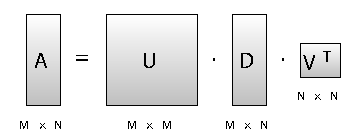
\includegraphics[width=0.75\textwidth]{img/svd_decomposition}
\end{figure}
\begin{itemize}
    \item $U$ is an $M\times M$ orthogonal matrix, $U^TU=I$
    \item $D$ is an $M\times N$ diagonal matrix
    \item $V^T$  is an $N\times N$ orthogonal matrix, $V^TV=I$ 
\end{itemize}
\subsection{Singular values}
The elements of $D$ are only non-zero on the diagonal and are called the \emph{singular values}. By convention, the order of the singular vectors is determined by the \emph{high-to-low} sorting of singular values, with the highest singular value in the upper left index of the $D$ matrix.
The first $r$ columns of $U$ are called \emph{left singular vectors}, they form an orthogonal basis for the space spanned by the columns of the original matrix $A$.

Similarly the first $r$ rows of $V^T$ are the \emph{right singular vectors}, they form an orthonormal basis for the row space of $A$.

SVD provides an explicit representation of the range and null-space of a matrix $A$.
\begin{itemize}
\item The right side singular vectors corresponding to vanishing singular values of $A$, span the null space of $A$:
\begin{align*}
d_i = 0 \quad \implies \quad Av_i = 0 \quad \implies \quad v_i \in Null(A).
\end{align*}
\item The left singular vectors corresponding to the non-zero singular values of $A$ span the range of $A$.
\end{itemize}
As a consequence, the rank of $A$ equals the number of non-zero singular values (= the number of non-zero elements in $D$).
\begin{align*}
Rank(A) = \# d_i > 0.
\end{align*}
\subsection{Closest Rank-$k$ Matrix}
Let the SVD of $A \in \R^{M\times N}$  be given by $A=UDV^T$. If $k<r = Rank(A)$ and
\begin{align*}
    A_k = \sum_{i=1}^k d_i u_i v_i^T.
\end{align*}
Then 
\begin{align*}
    \min_{Rank(B)=k} \norm{A-B}_2 = \norm{A-A_k}_2.
\end{align*}
This means that $A_k$ is the closest $Rank(k)$ approximation to $A$ in the Eculidean matrix norm sense hence:
\begin{align*}
    \norm{A-A_k}_2 = d_{k+1}.
\end{align*}

\subsection{Properties}
The columns of $U$ are the eigenvectors of $AA^T$. This claim can be verified using the SVD decomposition:
\begin{align*}
    AA^T = UDV^T VDU^T = UD^2U^T.
\end{align*}
Similarly the rows of $V^T$ (or columns of $V$) are the eigenvectors of $A^TA$ as:
\begin{align*}
    A^TA = VDU^T UDV^T = VD^2V^T.
\end{align*}

\subsection{Movie Example}
Let $A$ be a list of users with their respective movie preferences. Then the SVD decomposition
\begin{align*}
    A= UDV^T,
\end{align*}
can be interpreted in the following way:
\begin{itemize}
    \item $\mathbf{U}$: Users-to-concept affinity matrix.
    \item $\mathbf{D}$: Expression level of the different concepts in the data.
    \item $\mathbf{V}$: Movies-to-concept similarity matrix.
\end{itemize}


\begin{figure}[H]
    \centering
    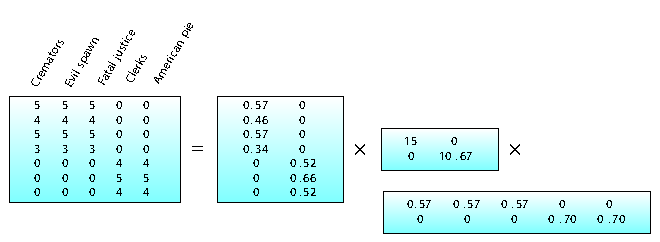
\includegraphics[width=\textwidth]{img/svd_movie}
\end{figure}
